\documentclass[11pt,a4paper]{article}
\usepackage[top=16mm,bottom=17mm,left=16mm,right=16mm,headheight=0pt,headsep=0mm,footskip=10mm]{geometry}
\usepackage{iftex}
\ifPDFTeX
  \usepackage[utf8]{inputenc}
  \usepackage[T5]{fontenc}
  \usepackage{mathptmx}
\else
  \usepackage{mathptmx}
  \usepackage{fontspec}
  \IfFontExistsTF{Times New Roman}{\setmainfont{Times New Roman}}{\IfFontExistsTF{TeXGyreTermes}{\setmainfont{TeXGyreTermes}}{\setmainfont{Latin Modern Roman}}}
\fi
\usepackage{amsmath,amssymb}
\usepackage{xcolor,tikz,enumitem,multicol,fancyhdr,lastpage}
\usepackage[most]{tcolorbox}
\definecolor{questionpurple}{RGB}{137,38,143}
\definecolor{answerblue}{RGB}{35,45,140}
\definecolor{lightblue}{RGB}{238,245,255}
\setlength{\parindent}{0pt}
\setlength{\parskip}{0pt}
\renewcommand{\baselinestretch}{1.10}
\setlength{\columnsep}{8mm}
\pagestyle{fancy}
\fancyhf{}
\renewcommand{\headrulewidth}{0pt}
\fancyfoot[L]{\small Chuyên đề III -- Toán 11}
\fancyfoot[R]{\small Trang \thepage/\pageref{LastPage} -- Bài 08}
\renewcommand{\footrulewidth}{.4pt}
\setlist[itemize]{leftmargin=6mm,label=\textcolor{answerblue}{\textbullet},itemsep=2pt,topsep=2pt,parsep=0pt}
\setlist[enumerate]{leftmargin=8mm,itemsep=2pt,topsep=2pt,parsep=0pt}
\newtcolorbox{theorybox}{colback=lightblue,colframe=answerblue!60,boxrule=.5pt,
  arc=1mm,left=2.5mm,right=2.5mm,top=1.5mm,bottom=1.5mm,before skip=3pt,after skip=4pt}
\newcommand{\sectitle}[2]{\vspace{4pt}\noindent{\large\bfseries\textcolor{questionpurple}{#1.\ #2}}\par\vspace{3pt}}
\newcommand{\exampletitle}[2]{\vspace{3pt}\noindent{\bfseries\textcolor{answerblue}{Ví dụ #1.}} #2\par\vspace{2pt}}
\newcommand{\propertytitle}[1]{\par\vspace{3pt}\noindent\textbf{\textcolor{answerblue}{#1}}\enspace}
\newcommand{\drawpoint}[3]{\fill[answerblue] (#1) circle (1.4pt) node[#2] {$#3$};}
\setlength{\abovedisplayskip}{5pt}
\setlength{\belowdisplayskip}{5pt}
\setlength{\abovedisplayshortskip}{3pt}
\setlength{\belowdisplayshortskip}{3pt}
\raggedbottom

\begin{document}
\noindent
\begin{minipage}[t]{.35\linewidth}
  \centering{\bfseries CHUYÊN ĐỀ III -- TOÁN -- 11\par}
  \vspace{2pt}\rule{.73\linewidth}{.4pt}\par\vspace{3pt}
  CHỦ ĐỀ 03\par\vspace{3pt}{\itshape TÀI LIỆU HỌC TẬP -- BÀI 08\par}
\end{minipage}\hfill
\begin{minipage}[t]{.62\linewidth}
  \centering{\bfseries HÌNH HỌC KHÔNG GIAN\par}
  \vspace{4pt}{\small\bfseries VẤN ĐỀ 11X32\par
  HAI ĐƯỜNG THẲNG SONG SONG\par}
\end{minipage}

\vspace{4mm}
\noindent\textbf{Họ và tên:}\dotfill\hfill\textbf{Lớp:}\enspace\dotfill
\vspace{2mm}

\begin{theorybox}
\textbf{Kiến thức trọng tâm:} Vị trí tương đối của hai đường thẳng trong
không gian; điều kiện để hai đường thẳng song song; các định lí về tính
song song và giao tuyến của ba mặt phẳng; vận dụng xác định giao tuyến
và giao điểm trong hình chóp, hình tứ diện.
\end{theorybox}

\sectitle{1}{Vị trí tương đối của hai đường thẳng}

Cho hai đường thẳng $a$ và $b$ trong không gian.
\begin{itemize}
  \item Nếu $a$ và $b$ cùng nằm trong một mặt phẳng, ta nói
  $a,b$ \textbf{đồng phẳng}. Khi đó chúng có thể \textbf{cắt nhau},
  \textbf{song song} hoặc \textbf{trùng nhau}.
  \item Nếu không có mặt phẳng nào cùng chứa $a$ và $b$ thì
  chúng \textbf{chéo nhau}; có thể nói $a$ chéo $b$ hoặc $b$ chéo $a$.
\end{itemize}
\begin{center}
\begin{minipage}[t]{.49\linewidth}\centering
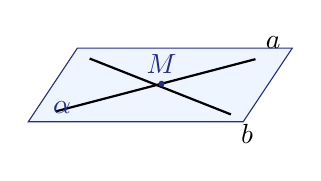
\begin{tikzpicture}[scale=.78]
  \fill[lightblue] (0,0)--(3.5,0)--(4.3,1.2)--(.8,1.2)--cycle;
  \draw[answerblue] (0,0)--(3.5,0)--(4.3,1.2)--(.8,1.2)--cycle;
  \draw[thick] (.45,.17)--(3.7,1.02) node[above right] {$a$};
  \draw[thick] (1.0,1.03)--(3.3,.12) node[below right] {$b$};
  \drawpoint{2.17,.62}{above}{M}
  \node[answerblue] at (.55,.24) {$\alpha$};
\end{tikzpicture}

{\small $a$ cắt $b$ tại $M$: $a\cap b=\{M\}$}
\end{minipage}\hfill
\begin{minipage}[t]{.49\linewidth}\centering
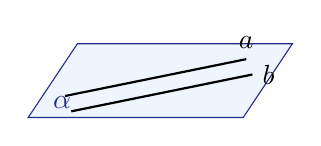
\begin{tikzpicture}[scale=.78]
  \fill[lightblue] (0,0)--(3.5,0)--(4.3,1.2)--(.8,1.2)--cycle;
  \draw[answerblue] (0,0)--(3.5,0)--(4.3,1.2)--(.8,1.2)--cycle;
  \draw[thick] (.6,.35)--(3.55,.95) node[above] {$a$};
  \draw[thick] (.7,.10)--(3.65,.70) node[right] {$b$};
  \node[answerblue] at (.55,.25) {$\alpha$};
\end{tikzpicture}

{\small $a$ song song $b$: $a\parallel b$}
\end{minipage}

\vspace{2mm}
\begin{minipage}[t]{.49\linewidth}\centering
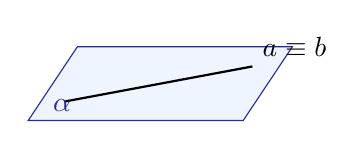
\begin{tikzpicture}[scale=.78]
  \fill[lightblue] (0,0)--(3.5,0)--(4.3,1.2)--(.8,1.2)--cycle;
  \draw[answerblue] (0,0)--(3.5,0)--(4.3,1.2)--(.8,1.2)--cycle;
  \draw[thick] (.6,.31)--(3.65,.88) node[above right] {$a\equiv b$};
  \node[answerblue] at (.55,.25) {$\alpha$};
\end{tikzpicture}

{\small $a$ trùng $b$: $a\equiv b$}
\end{minipage}\hfill
\begin{minipage}[t]{.49\linewidth}\centering
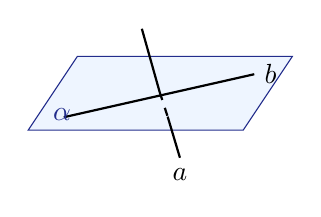
\begin{tikzpicture}[scale=.78]
  \fill[lightblue] (0,0)--(3.5,0)--(4.3,1.2)--(.8,1.2)--cycle;
  \draw[answerblue] (0,0)--(3.5,0)--(4.3,1.2)--(.8,1.2)--cycle;
  \draw[thick] (.58,.21)--(3.68,.91) node[right] {$b$};
  \draw[thick] (1.85,1.65)--(2.14,.62);
  \draw[thick,dashed] (2.14,.62)--(2.27,.22);
  \draw[thick] (2.27,.22)--(2.47,-.45) node[below] {$a$};
  \node[answerblue] at (.55,.25) {$\alpha$};
\end{tikzpicture}

{\small $a$ và $b$ chéo nhau}
\end{minipage}
\end{center}

\begin{theorybox}
\textbf{Định nghĩa.} Hai đường thẳng \textbf{song song} là hai đường thẳng
\textbf{đồng phẳng} và \textbf{không có điểm chung}:
\[
  \boxed{a\parallel b\quad\Longleftrightarrow\quad
  a,b\text{ đồng phẳng và }a\cap b=\varnothing.}
\]
\end{theorybox}

\begin{itemize}
  \item Có đúng \textbf{một mặt phẳng} chứa hai đường thẳng song song
  $a,b$; kí hiệu mặt phẳng đó là $(a,b)$.
  \item Trong không gian, hai đường thẳng không có điểm chung thì
  \textbf{hoặc song song, hoặc chéo nhau}; không thể chỉ dựa vào
  việc không có điểm chung để kết luận chúng song song.
  \item Trong tứ diện $ABCD$, các cặp cạnh đối
  $AB,CD$; $AC,BD$; $AD,BC$ đều chéo nhau.
\end{itemize}

\begin{center}
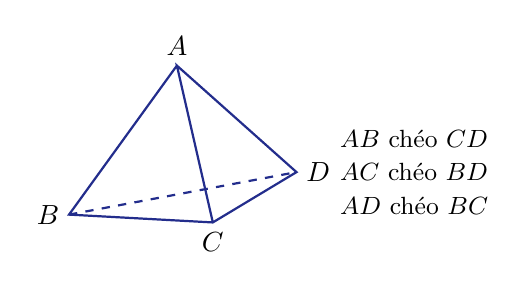
\begin{tikzpicture}[scale=.83]
  \coordinate (A) at (1.65,2.28);
  \coordinate (B) at (0,0);
  \coordinate (C) at (2.2,-.12);
  \coordinate (D) at (3.48,.65);
  \draw[answerblue,thick] (A)--(B)--(C)--(D)--(A)--(C);
  \draw[answerblue,thick,dashed] (B)--(D);
  \node[above] at (A) {$A$};
  \node[left] at (B) {$B$};
  \node[below] at (C) {$C$};
  \node[right] at (D) {$D$};
  \node[right,align=left] at (4,.65)
    {\small $AB$ chéo $CD$\\[-1pt]\small $AC$ chéo $BD$\\[-1pt]\small $AD$ chéo $BC$};
\end{tikzpicture}
\end{center}

\textbf{Ví dụ minh họa.} Xét hình chóp $S.ABCD$ có đáy $ABCD$
là hình bình hành.
\begin{center}
\begin{tikzpicture}[scale=.9]
  \coordinate (A) at (.95,.82); \coordinate (B) at (0,0);
  \coordinate (C) at (2.65,0); \coordinate (D) at (3.6,.82);
  \coordinate (S) at (1.55,2.75);
  \draw[answerblue,thick] (S)--(B)--(C)--(D)--(S)--(C);
  \draw[answerblue,dashed] (S)--(A)--(B) (A)--(D);
  \node[above] at (S) {$S$};
  \node[left] at (A) {$A$};
  \node[left] at (B) {$B$};
  \node[below] at (C) {$C$};
  \node[right] at (D) {$D$};
  \node[right,align=left] at (4.1,1.15)
  {\small $AB\parallel CD,\quad AD\parallel BC$\\[3pt]
   \small $SA$ chéo với $BC$ và $CD$};
\end{tikzpicture}
\end{center}

\sectitle{2}{Tính chất}

\propertytitle{Định lí 1.}
Trong không gian, qua một điểm không nằm trên đường thẳng cho trước,
có đúng \textbf{một đường thẳng} song song với đường thẳng đã cho.

\begin{center}
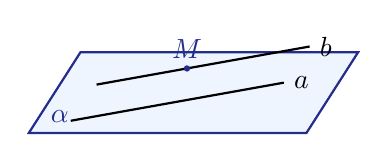
\begin{tikzpicture}[scale=.82]
  \fill[lightblue] (0,0)--(4.3,0)--(5.1,1.25)--(.8,1.25)--cycle;
  \draw[answerblue,thick] (0,0)--(4.3,0)--(5.1,1.25)--(.8,1.25)--cycle;
  \draw[thick] (.65,.19)--(3.95,.78) node[right] {$a$};
  \draw[thick] (1.05,.75)--(4.35,1.34) node[right] {$b$};
  \drawpoint{2.45,1.00}{above}{M}
  \node[answerblue] at (.48,.25) {$\alpha$};
\end{tikzpicture}
\end{center}

\begin{itemize}
  \item Nếu $a\subset(\alpha)$, $M\in(\alpha)$ và $M\notin a$,
  thì đường thẳng $b$ đi qua $M$ và song song với $a$ cũng nằm trong
  $(\alpha)$:
  \[
     \boxed{a\subset(\alpha),\ M\in(\alpha),\ M\notin a,\quad
      b\ni M,\ b\parallel a\ \Longrightarrow\ b\subset(\alpha).}
  \]
  \item Cho mặt phẳng $(ABC)$ và $AD\parallel BC$. Khi đó
  $D\in(ABC)$, nên
  \[
     \boxed{(ABC)\equiv(ABCD).}
  \]
\end{itemize}
\begin{center}
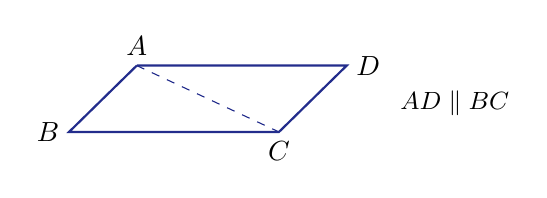
\begin{tikzpicture}[scale=.86]
  \coordinate (A) at (1,.98);
  \coordinate (B) at (0,0);
  \coordinate (C) at (3.1,0);
  \coordinate (D) at (4.1,.98);
  \draw[answerblue,thick] (A)--(B)--(C)--(D)--(A);
  \draw[answerblue,dashed] (A)--(C);
  \node[above] at (A) {$A$};
  \node[left] at (B) {$B$};
  \node[below] at (C) {$C$};
  \node[right] at (D) {$D$};
  \node[right] at (4.75,.43) {\small $AD\parallel BC$};
\end{tikzpicture}
\end{center}

\propertytitle{Định lí 2.}
Nếu ba mặt phẳng đôi một cắt nhau theo \textbf{ba giao tuyến phân biệt}
thì ba giao tuyến ấy \textbf{hoặc đồng quy, hoặc song song với nhau}.

\begin{center}
\begin{minipage}[t]{.49\linewidth}\centering
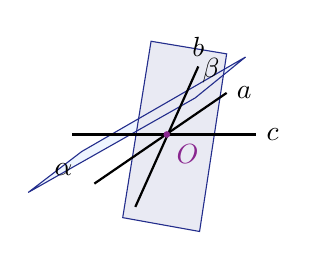
\begin{tikzpicture}[scale=.8]
  \fill[lightblue] (0,.2)--(2.65,1.7)--(3.45,2.35)--(.85,.85)--cycle;
  \fill[answerblue!10] (1.5,-.2)--(1.95,2.6)--(3.15,2.4)--(2.72,-.42)--cycle;
  \draw[answerblue] (0,.2)--(2.65,1.7)--(3.45,2.35)--(.85,.85)--cycle;
  \draw[answerblue] (1.5,-.2)--(1.95,2.6)--(3.15,2.4)--(2.72,-.42)--cycle;
  \coordinate (O) at (2.2,1.12);
  \draw[thick] (1.05,.34)--(3.15,1.78) node[right] {$a$};
  \draw[thick] (1.7,-.03)--(2.7,2.2) node[above] {$b$};
  \draw[thick] (.7,1.12)--(3.62,1.12) node[right] {$c$};
  \fill[questionpurple] (O) circle (1.5pt) node[below right] {$O$};
  \node at (.56,.56) {$\alpha$};\node at (2.9,2.14) {$\beta$};
\end{tikzpicture}

{\small Ba giao tuyến đồng quy (minh họa)}
\end{minipage}\hfill
\begin{minipage}[t]{.49\linewidth}\centering
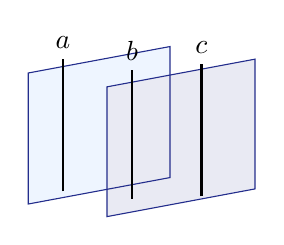
\begin{tikzpicture}[scale=.8]
  \fill[lightblue] (0,0)--(2.25,.42)--(2.25,2.5)--(0,2.08)--cycle;
  \fill[answerblue!10] (1.25,-.2)--(3.6,.24)--(3.6,2.3)--(1.25,1.86)--cycle;
  \draw[answerblue] (0,0)--(2.25,.42)--(2.25,2.5)--(0,2.08)--cycle;
  \draw[answerblue] (1.25,-.2)--(3.6,.24)--(3.6,2.3)--(1.25,1.86)--cycle;
  \draw[thick] (.55,.2)--(.55,2.3) node[above] {$a$};
  \draw[thick] (1.65,.08)--(1.65,2.12) node[above] {$b$};
  \draw[thick] (2.75,.12)--(2.75,2.22) node[above] {$c$};
\end{tikzpicture}

{\small Ba giao tuyến song song (minh họa)}
\end{minipage}
\end{center}

\begin{theorybox}
\textbf{Hệ quả.} Nếu hai mặt phẳng \textbf{phân biệt} lần lượt chứa
hai đường thẳng song song thì giao tuyến của chúng (nếu có)
\textbf{hoặc song song với cả hai đường thẳng đó, hoặc trùng với
một trong hai đường thẳng đó}.
\end{theorybox}

\propertytitle{Định lí 3.}
Trong không gian, \textbf{hai đường thẳng phân biệt cùng song song với
một đường thẳng thứ ba thì song song với nhau}:
\[
  \boxed{a\parallel c,\quad b\parallel c,\quad a\ne b
   \quad\Longrightarrow\quad a\parallel b.}
\]
\begin{center}
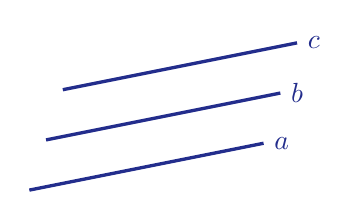
\begin{tikzpicture}[scale=.85]
 \draw[answerblue,very thick] (0,0)--(3.5,.7) node[right] {$a$};
 \draw[answerblue,very thick] (.25,.75)--(3.75,1.45) node[right] {$b$};
 \draw[answerblue,very thick] (.5,1.5)--(4,2.2) node[right] {$c$};
\end{tikzpicture}
\end{center}

\sectitle{3}{Ví dụ vận dụng}

\exampletitle{01 [TDM31]}{Cho hình chóp $S.ABCD$ có đáy $ABCD$
là hình thang với hai đáy là $AB$ và $CD$. Gọi $M$ là điểm
thuộc cạnh $SB$.}
\begin{enumerate}
  \item Hãy xác định giao tuyến của hai mặt phẳng $(SAB)$ và $(SCD)$.
  \item Hãy xác định giao điểm của $SA$ và $(CDM)$.
\end{enumerate}

\exampletitle{02 [TDM31]}{Cho tứ diện $ABCD$. Gọi $M,N$ lần lượt
là trung điểm của $AB,AC$. Mặt phẳng $(\alpha)$ đi qua $M,N$
và cắt các cạnh $DC,DB$ lần lượt tại $P,Q$.
Hỏi tứ giác $MNPQ$ là hình gì?}

\vspace{2mm}
\begin{tcolorbox}[colback=white,colframe=black!35,boxrule=.4pt,arc=0mm,
 left=2mm,right=2mm,top=1mm,bottom=1mm]
\footnotesize
\textbf{Nguồn nội dung:} TƯ DUY MỞ,
\emph{Vấn đề 11X32: Hai đường thẳng song song},
biên soạn Nguyễn Đăng Ái, trang 1--3 (PDF được cung cấp).
Đã biên tập lại thành LaTeX, vẽ lại hình minh họa, loại bỏ
ô trống làm bài, quảng cáo và nền giấy kẻ.
Bản gốc không có lời giải chi tiết cho hai ví dụ; bản này giữ nguyên câu hỏi.
\end{tcolorbox}
\end{document}
